\part{Kiosk}
\label{kiosk}

\chapter{Structuur}
\label{kiosk:structuur}

De manier waarop we de kioskapplicatie hebben opgedeeld kent sterke gelijkenissen met de manier waarbij we de serverapplicatie gestructureerd hebben: alle logische componenten (het netwerk subsysteem, de datamanager en de userinterface) worden geïsoleerd in een apart subsysteem, en een overkoepelende controller staat in voor interacties die over verschillende subsystemen heen gaan.

\section{Netwerk subsysteem}
\label{kiosk:structuur:netwerk}

Dit gedeelte van de applicatie neemt alle netwerkcommunicatie op zich. Daartoe creëert het een \ac{upnp} device, registreert het de nodige services, en broadcast het die gegevens. Wanneer een bepaalde actie aangeroepen wordt, zal de respectievelijke service louter een signaal uitsturen. Dat signaal (bijvoorbeeld \code{reboot} of \code{setVolume(uint)}) zal vervolgens opgevangen worden door de applicatiecontroller, die dan tot de effectieve actie overgaat.

Door de effectieve implementatie in een andere klasse te plaatsen vereenvoudigen we de netwerkinterface die in de minimale opzet al complex genoeg is (beheren van \ac{upnp} state variables, conversie van parameters, registratie van \ac{scpd} bestanden, \ldots). Tevens wordt de hele component hierdoor platform-onafhankelijk, en moeten we bij het herimplementeren voor een nieuw platform enkel de implementatie herschrijven die volledig geïsoleerd is binnen de applicatiecontroller. Dit is opnieuw vergelijkbaar met de opzet die we gehanteerd hebben bij de serverapplicatie: code binnen een bepaald subsysteem staat enkel in voor verwerking relevant voor dat subsysteem, acties die ergens anders een impact hebben worden afgehandeld door de applicatiecontroller.

\subsection{Datamanager}
\label{kiosk:structuur:datamanager}

Deze klasse komt overeen met het repository subsysteem in de serverapplicatie, maar heeft een andere naam gekregen wegens een \emph{namespace clash} met enkele klassen die we gebruiken uit een library. De taken veranderen echter niet: de datamanager staat in  voor het ophalen van gegevens die zich in een externe \ac{svn} repository bevinden, en alles dat daarmee gepaard gaat. Zo zal de component moeten rekening houden met een eventuele cache, om zo een checkout van gegevens te versnellen. Ook moet het bij het opstarten kunnen controleren of er geen oude checkout aanwezig is, om zo direct al een voorstelling te kunnen weergeven, zelfs als dat een oude voorstelling betreft.

In tegenstelling tot de repository klasse in de serverapplicatie moeten we hier geen data interpreteren: na een checkout of update gedaan te hebben, moet de voorstelling in zijn geheel opnieuw doorgegeven worden aan de userinterface, het is niet van belang om te weten wélke gegevens veranderd zijn. Hierdoor wordt het gebruik van de \ac{svn} libraries sterk vereenvoudigd.

% backup cache uitleggen? config saven enzo

\subsection{Userinterface}
\label{kiosk:structuur:userinterface}

Dit gedeelte van de applicatie staat in voor de effectieve weergave van ontvangen voorstellingen. Zoals reeds vermeld bestaan die voorstellingen uit \ac{html} en Javascript, en gebruiken we de WebKit rendering engine om die gegevens weer te geven. In de huidige opzet hebben we enkel voorzien in een naadloze integratie van de rendering engine en onze applicatie, waardoor de voorstellingen zeer vlot geladen en verwerkt kunnen worden. Voor een volgende versie plannen we de uitbreiding van deze component zodat deze niet alleen voorstellingen weergeeft, maar gegevens over hoe exact die weergegeven worden, teruggestuurd worden naar de server. Zo kunnen we bijvoorbeeld statistieken vergaren over welke voorstellingen het meest bekeken worden, welke filmpjes het snelst gestopt worden, \ldots

Omdat de integratie van de rendering engine en de rest van de applicatie zo goed bleek te werken, hebben we besloten om de overige gebruikersinterfaces op eenzelfde manier te implementeren in \ac{html} en Javascript. Hoewel er niet zoveel reguliere interfaces binnen de applicatie te vinden zijn (opstart-pagina, en enkele debug pagina's), resulteerde dit in een uniforme userinterface-implementatie waarbij het zelfs op termijn mogelijk zou moeten zijn om de interface code dynamisch te updaten op eenzelfde manier als dat bij de voorstellingen gebeurt.

Er is echter een groot verschil tussen een ordinaire voorstelling en een userinterface-pagina bij de applicatie: waar een voorstelling volledig \emph{self-contained} is, heeft een informatieve userinterface-pagina gegevens nodig uit de applicatie. Een debugpagina bijvoorbeeld heeft nood aan een mechanisme om debuggegevens van de applicatie te ontvangen.
Een mogelijkheid zou zijn om via \ac{ajax} gegevens op te halen die via een webservice lokaal opengesteld worden. Dit verhoogt echter de complexiteit van zowel de interface als de kioskapplicatie, laat staan dat het een efficiënte manier is om een weinig gegevens over te brengen. Daarom hebben we gekozen voor een secundaire piste, waarbij we gebruik maken van de \makeurl{http://doc.qt.nokia.com/latest/qtwebkit-bridge.html}{QtWebKit Bridge}. Dit mechanisme laat ons toe om een klasse binnen onze C++ applicatie toegankelijk te maken vanuit Javascript code, om zo gegevens op een efficiënte manier te kunnen doorspelen. Zo hebben we voor alle soorten pagina's die we moeten kunnen weergeven, een meta-klasse aangemaakt die de nodige gegevens aggregeert (zie fragment \ref{lst:expose_cpp}). Bij het aanmaken van de pagina in kwestie wordt die meta-klasse vervolgens geregistreerd binnen de rendering engine, waardoor de Javascript code die met de pagina geladen wordt er toegang tot heeft. Een voorbeeld van dit laatste is te zien in fragment \ref{lst:expose_js}.

\begin{lstlisting}[language=C++, float, caption=Registratie van een klasse binnen de rendering engine., label=lst:expose_cpp]
class LogPage : public QWebPage
{
Q_OBJECT
Q_PROPERTY(QString id READ id CONSTANT)
public:
    LogPage(QObject* parent = 0);
    ~LogPage();

    QString id() const;
signals:
    void newMessage(const QString& iMessage);
};

LogPage::LogPage(QObject *parent) : QWebPage(parent)
{
    mainFrame()->addToJavaScriptWindowObject(
    	"application",
        this);
}
\end{lstlisting}

\begin{lstlisting}[language=JavaScript, float, caption=Gebruik van een geregistreerde C++ klasse., label=lst:expose_js]
// Gebruik van een signaal
function showMessage(message) { }
application.newMessage.connect(showMessage);

// Gebruik van een property
document.write(application.id)
\end{lstlisting}


\chapter{Realisatie}
\label{kiosk:realisatie}

Tijdens de realisatie van de kioskapplicatie zijn we op enkele interessante problemen gestuit die zeker het vermelden waard zijn.

\section{Uniek ID}
\label{kiosk:realisatie:id}

Aangezien de software die op de kiosken zal draaien volledig identiek is -- we streven immers naar een configuratieloze opzet -- moet de applicatie in staat zijn om een identifier te genereren die uniek is, maar toch gebonden aan een specifieke kiosk om er vanuit de configuratie naar te kunnen verwijzen. De identifier zal gebruikt worden door de \ac{upnp} library, die het doorspeelt naar een externe partij als deel van de device description. Daarom zullen we ons moeten schikken naar de \ac{upnp} standaard, die een \ac{uuid} vereist als identifier.

Een \ac{uuid} is zeer specifiek opgemaakt, en bestaat steeds uit 16 bytes, onderverdeeld in 5 groepen die elk gescheiden zijn door een steepje: \code{DEADBEEF-E29B-41D4-A716-446655440000}. Er bestaan echter verschillende \ac{uuid} varianten, elk met een aantal versies. Zowel de variant als de versie wordt in de \ac{uuid} string geëncodeerd, met als template \code{xxxxxxxx-xxxx-Mxxx-Nxxx-xxxxxxxxxxxx}. De officiële specificatie detailleert maar 1 variant, die geïdentificeerd wordt door de twee meest-significante bits van de \code{N} byte op $1 0$ in te stellen. Betreffende de versie hebben we de keus uit een aantal versies, en kiezen we voor een gewijzigde vorm van de \ac{mac} versie. Hierbij moet de \code{M} byte ingesteld worden op een hexadecimale 1, en kunnen we de eerste twee groepen (samen exact 12 bytes) gebruiken om het \ac{mac} adres in te encoderen.

Normaal worden de overige bits vervolgens gevuld met tijdsgegevens, maar omdat we willen dat onze identifier identiek blijft na een reboot kiezen we ervoor om die bits op 0 in te stellen. Het resultaat hiervan valt te vinden in fragment \ref{lst:uuid}.

\begin{lstlisting}[language=C++, float, caption=Generatie van een \acs{uuid}., label=lst:uuid]
QUuid getHardwareUuid() const
{
  // Maak een interface request object aan
  struct ifreq tRequest;
  bzero(&tRequest, sizeof(tRequest));
  tRequest.ifr_addr.sa_family = AF_INET;
  strncpy(tRequest.ifr_name, "eth0", IFNAMSIZ-1);

  // Open een socket en voer de systeemaanroep uit
  int tFd = socket(AF_INET, SOCK_DGRAM, 0);
  ioctl(tFd, SIOCGIFHWADDR, &tRequest);
  close(tFd);

  // Genereer een UUID
  char* tMAC = ifr.ifr_hwaddr.sa_data
  QUuid oUuid;
  oUuid.data1    |= (unsigned char) tMAC[0] << 24;
  oUuid.data1    |= (unsigned char) tMAC[1] << 16;
  oUuid.data1    |= (unsigned char) tMAC[2] << 8;
  oUuid.data1    |= (unsigned char) tMAC[3];
  oUuid.data2    |= (unsigned char) tMAC[4] << 8;
  oUuid.data2    |= (unsigned char) tMAC[5];
  oUuid.data4[0]  = (oUuid.data4[0] & 0x3F  ) | 0x80;
  oUuid.data3     = (oUuid.data3    & 0x0FFF) | 0x1000;
  
  return oUuid;
}
\end{lstlisting}

\section{BRisa \acs{upnp} library}
\label{kiosk:realisatie:brisa}

Zoals reeds vermeld gebruiken we de BRisa library aan de kant van de kiosk, waarbij acties en methodes opgeroepen worden door de Cling bibliotheek aan de kant van de server. Cling staat er echter voor bekend om de \ac{upnp} specificatie op de letter te volgen, waarbij elke afwijking daarvan als een waarschuwing of zelfs vaak als een regelrechte fout beschouwd wordt. En jammer genoeg bleek de BRisa bibliotheek soms laks om te gaan met de standaarden voorgeschreven door de \ac{upnp} standaard \ldots

Om Cling te overtuigen om zonder veel probleem te werken met clients die de BRisa bibliotheek gebruiken, hebben we twee patches moeten doorvoeren. De eerste daarvan introduceert een extra spatie voor het \code{s:encodingStyle} attribuut dat meegestuurd wordt bij elk \ac{soap} bericht. Zonder deze spatie weigerde Cling de antwoorden van de BRisa bibliotheek te verwerken, waardoor het niet mogelijk was om acties uit te voeren. Een tweede patch voegt de optionele \code{content-type} header toe aan berichten waarbij de ontwikkelaars van BRisa dat vergeten waren, waardoor Cling nu ook zonder waarschuwingen kan communiceren met een BRisa server.

Hierbij was het een groot voordeel dat de library open-source was. Nadat we het probleem gelocaliseerd hadden door de foutmeldingen van Cling te combineren met een analyse van de verzonden berichten, konden we eenvoudig de code van de library ophalen, het probleem localiseren en oplossen. Hoewel we beide patches ingestuurd hebben op de bug tracker van het BRisa project (\makeurl{https://garage.maemo.org/tracker/index.php?func=detail\&aid=6953\&group\_id=138\&atid=583}{eerste patch}, \makeurl{https://garage.maemo.org/tracker/index.php?func=detail\&aid=6954\&group\_id=138\&atid=583}{tweede patch}), kon het gerust nog even duren vooraleer de wijzigingen toegepast werden, of dat een nieuwe versie zou vrijgegeven worden. Daarom hebben we een \makeurl{https://github.com/MIRAvzw/qt-brisa}{onze eigen versie} van het project gemaakt (ook wel een \emph{fork}) genoemd, waarin de fouten reeds gecorrigeerd zijn. Op de toestellen waarop de applicatie ontwikkeld en geïnstalleerd wordt kunnen we nu in afwachting van een nieuwe versie onze eigen versie van de bibliotheek installeren.

\section{svnqt \acs{svn} library}
\label{kiosk:realisatie:svnqt}

Zoals beschreven in hoofdstuk \ref{ontwerp} hebben we voor onze kioskapplicatie een interessante \ac{svn} library gevonden die gebruik maakt en geïntegreerd is met het Qt framework dat we gebruiken. De code was oorspronkelijk een stand-alone library, genaamd ``svncpp" en ontwikkeld door RapidSVN in 2002. Nadien is de code geïntegreerd en verder ontwikkeld als deel van de KDESvn applicatie. Om de code eenvoudig doch efficiënt te kunnen gebruiken binnen onze kioskapplicatie hebben we code uit de KDESvn applicatie geëxtraheerd en er een \makeurl{https://github.com/MIRAvzw/svnqt}{alleenstaande bibliotheek} van gemaakt. Buiten enkele kleine ingrepen waren er verder geen aanpassingen nodig om deze code vervolgens te kunnen gebruiken binnen ons project.

\section{Log4qt library}
\label{kiosk:realisatie:log4qt}

Log4qt is een project dat een Log4J-achtige interface aanbiedt om op eenvoudige manier een consistente logging te voorzien, waarbij het mogelijk is om via een configuratiebestand te specificeren waar de logberichten terechtkomen (zoals te zien is in fragment \ref{lst:log4qt}). Hoewel de bibliotheek functioneel vrij compleet is en op het eerste zicht geen problemen opleverde, hebben we naar verloop van tijd toch enkele wijzigingen toegebracht aan de \emph{upstream} code.

\begin{lstlisting}[language=JavaProperties, float, caption=Externe configuratie van Log4qt., label=lst:log4qt]
# Registreer alle appenders
log4j.rootLogger          = DEBUG, dbg

# Debug appender
log4j.appender.dbg        = org.apache.log4j.FileAppender
log4j.appender.dbg.file   = debug.log
log4j.appender.dbg.layout = org.apache.log4j.TTCCLayout
\end{lstlisting}

Een \makeurl{https://gitorious.org/log4qt/log4qt/merge\_requests/3}{eerste patch} die we ingestuurd hebben corrigeerde een probleem met namespaces. C++ code die gebruik maakt van Qt wordt immers eerst gepreprocessed door een Qt-specifieke preprocessor: de \ac{moc}. Deze preprocessor zorgt ervoor dat Qt meta-objecten en introspectiemogelijkheden krijgt, wat krachtige mechanismen zoals \code{signals \& slots} mogelijk maakt. Dit mechanisme is echter niet altijd even robuust: externe factoren kunnen ertoe leiden dat een \ac{moc}-macro verkeerd expandeert, en dat was hier het geval bij een ontbrekende namespace prefix binnen een \code{Q\_PROPERTY} \ac{moc}-macro.

Vervolgens hebben we ook enkele kleine features toegevoegd die het werken met de bibliotheek aangenamer maken. Zo hebben we voorzien in een \makeurl{https://gitorious.org/log4qt/log4qt/merge\_requests/4}{patch} die het mogelijk maakt om de Log4qt objecten te gebruiken met output operatoren: dit is een veelgebruikte techniek in de officiële Qt libraries waardoor de Log4qt bibliotheek eenvoudiger is voor mensen die er nog niet thuis in zijn maar toch ervaring hebben met Qt. Op vergelijkbare wijze hebben we de manier om headers te includen \makeurl{https://gitorious.org/log4qt/log4qt/merge\_requests/5}{gewijzigd} zodat het eveneens dichter aanleunt bij de manier waarop dat gebeurt bij de officiële Qt code.

\section{Statische codeanalyse}
\label{kiosk:realisatie:codeanalyse}

Net zoals we dat bij de serverapplicatie gedaan hebben, willen we met behulp van statische codeanalyse proberen de kwaliteit van de code te verbeteren. Jammer genoeg blijkt het voor C++ code veel moeilijker te zijn om aan statische analyse te doen. Het grote probleem is dat van de \emph{preprocessor}: door toe te laten dat macro's op een heel flexibele manier arbitraire code kunnen genereren is het veel moeilijker om eenduidig op zoek te gaan naar fouten in die code. Zeker in het geval van Qt, dat sterk berust op macro's om geavanceerde technieken zoals signalen en introspectie te implementeren.

\subsection{Stijl}
\label{kiosk:realisatie:codeanalyse:stijl}

Na lang gezocht te hebben bleek er geen goede tool te bestaan om de stijl van een C++ codebase te controleren, wat we bij de serverapplicatie wel hebben kunnen doen met Checkstyle. Het beste dat we gevonden hebben is \makeurl{https://google-styleguide.googlecode.com/svn/trunk/cpplint/cpplint.py}{cpplint}, een script door Google ontworpen dat ze intern gebruiken om hun C++ code te standaardiseren. Maar zoals nogal snel duidelijk werd is het een veel minder krachtige applicatie: het voert enkel wat rudimentaire controles uit op vlak van indentatie en andere elementaire syntax, geavanceerde modules zoals Checkstyle ze kent, vinden we hier niet terug. Gelukkig is de kioskapplicatie een pak minder complex dan de serverapplicatie, waardoor het toch nog haalbaar is om de code af en toe manueel te overlopen.

\subsection{Correctheid}
\label{kiosk:realisatie:codeanalyse:correctheid}

Om de correctheid van C++ code te analyseren bestaan er al wat meer tools, zoals het veelgebruikte en relatief uitgebreide \makeurl{http://cppcheck.sourceforge.net/}{cppcheck}. Deze tool controleert onder andere het gebruik van arrays, of excepties correct afgehandeld worden, en of er geen grote memory leaks zijn. Dankzij deze applicatie hebben we verschillende codefragmenten kunnen identificeren waar objecten onnodig gekopiëerd werden, wat het geheugengebruik ten goede gekomen is.

Een probleem met cppcheck is dat het niet goed overweg kan met de vele macro's specifiek aan Qt. Daarom zijn we op zoek gegaan naar een statische codeanalysetool die op zijn minst geen problemen heeft met de constructies die we terugvinden bij Qt applicaties. En zo een tool hebben we ook gevonden, onder de naam \makeurl{http://www.englishbreakfastnetwork.org/krazy/}{Krazy}. Deze applicatie is deel van het \ac{kde} project, een desktop environment die hoofdzakelijk bestaat uit Qt en C++. Krazy is dan ook specifiek gemaakt om niet alleen overweg te kunnen met Qt code, maar om ze ook expliciet te controleren op fouten. Hoewel Krazy veel onbelangrijke problemen vermeldde (die vaak hun oorsprong kennen in de \ac{kde} coding policies), heeft het ook effectief een serieuze fout gevonden. Bij een bepaalde klasse hadden we immers een essentiële macro vergeten die absoluut nodig is om een correct object te verkrijgen.

\chapter{Deployment}
\label{kiosk:deployment}

\section{Besturingssysteem}
\label{kiosk:deployment:besturingssysteem}

Zoals vermeld in \ref{server:deployment:besturingssysteem} was het voor de serverapplicatie niet haalbaar om te switchen naar een krachtiger besturingssysteem wegens verschillende hardwarebeperkingen. Bij de meer \emph{general-purpose} hardware die we voor de kiosken gekocht hebben, is dit anders: het toestel komt met een \ac{sd} kaartslot, en het is met de standaard bootloader zelfs mogelijk om op te starten van een besturingssysteem dat zich op zo een geheugenkaart bevindt. Hierdoor kunnen we veel gemakkelijker een alternatief besturingssysteem ontwikkelen, omdat er nu snel gedeployed kan worden naar een \ac{sd} kaartje dat we dan ook zonder gevaar op beschadiging direct kunnen uittesten op het toestel. Ook hebben we bij de aankoop gevraagd om er een \emph{debug interface chip} bij te krijgen, waarmee we een seriële interface kunnen aankoppelen zodat we al heel vroeg in het opstartproces zicht hebben op informatieve berichten, en toegang hebben tot een \ac{jtag} connector om in het geval van een beschadiging toch nog de geheugenchips te kunnen herprogrammeren.

\subsection{Distributie}
\label{kiosk:deployment:besturingssysteem:distributie}

Aangezien de Efika MX enkel Linux ondersteunt, zullen we een besturingssysteem moeten gebruiken dat daarmee compatibel is. In principe zou het mogelijk zijn om enkel te vertrekken van de Linux kernel, en de nodige \emph{userspace} volledig zelf samen te stellen. Dat is echter een zeer groot werk, waarmee we ook een zeer rigide eindproduct krijgen. Daarom gaan we uit van een bestaande distributie, die we vervolgens aan onze eigen noden zullen aanpassen. Het zou bovendien handig zijn moesten die aanpassingen op een gestructureerde manier kunnen verlopen, liefst via een of ander beheersysteem.

Vooreerst hebben we natuurlijk gekeken naar het besturingssysteem dat reeds geïnstalleerd is op de hardware: een variant van Ubuntu 10.10. Het probleem met deze distributie is dat ze sterk geoptimaliseerd is voor het gebruik als een desktop-computer (de Efika MX wordt geadverteerd als een \emph{cloud computer}), waardoor het veel voor ons nutteloze pakketten en configuraties bevat. We zouden in principe wel alles kunnen verwijderen wat we niet nodig hebben, maar dit is een langdradig en foutgevoelig proces waarbij we uiteindelijk toch altijd wel iets zullen vergeten.

Daarom hebben we gekozen om uit te gaan van een \makeurl{http://www.debian.org/}{Debian} basissysteem, omdat Debian een zeer goed gestructureerd en krachtig pakketbeheersysteem kent (\code{dpkg}) en zelfs verschillende tools voorziet om ook de samenstelling van het basissysteem te kunnen veranderen (\code{debootstrap} en \code{multistrap}). Ook bestaan er veel varianten van Debian die misschien zelfs nog dichter aanleunen bij onze specifieke eisen.

\subsection{Kernel}
\label{kiosk:deployment:besturingssysteem:kernel}

Aangezien de Linux kernel valt onder de \ac{gpl} licentie moet Genesi alle wijzigingen nodig om Linux op de Efika MX te laten draaien vrijgegeven onder dezelfde licentie. Jammer genoeg zijn die wijzigingen nog niet geïntegreerd in de \emph{mainline kernel}, en onderhoudt Genesi \makeurl{git://gitorious.org/efikamx/linux-kernel.git}{een eigen fork} van Linux. Dit is vervelend omdat we daarom niet de laatste kernel kunnen gebruiken, maar ons moeten houden aan de versie die Genesi publiceert. Ook is het moeilijker om extra modules of patches te gebruiken omdat die meestal gebaseerd zijn op de mainline kernel.

We hebben er voor gekozen om de kernel te hergebruiken die Genesi voorziet bij de distributie die standaard op de Efika MX geïnstalleerd is. Hierbij sparen we ons het werk uit om zelf Linux te configureren en compileren, en kunnen we erop vertrouwen dat de configuratie correct en stabiel is. Om de kernel te hergebruiken hebben we een aantal bestanden moeten extraheren. Het belangrijkste bestand is daarbij natuurlijk de kernel zelf: \code{/boot/uImage}. Maar Genesi heeft hun kernel zodanig geconfigureerd dat code die optionele functionaliteit voorziet niet in de kernel zelf gecompileerd is, maar afgesplitst wordt in externe modules. Het probleem hierbij is dat sommige van die modules reeds nodig zijn tijdens het opstarten (denken we bijvoorbeeld aan de modules die voorzien in de implementatie van het bestandssysteem), waardoor we ze niet zomaar op de root partitie van het besturingssysteem kunnen plaatsen. Een oplosssing hiervoor is om de modules te verpakken in een image die samen met de kernel in het \ac{ram} geheugen ingeladen wordt wanneer de computer opstart. Dit bestand, ook wel de \emph{initial ramdisk} genoemd, vinden we terug onder \code{/boot/uInitrd}. Een laatste groep bestanden die we moeten kopiëren vinden we in de map \code{/lib/firmware}: dit zijn firmware bestanden die nodig zijn om bepaalde hardware te kunnen gebruiken. Aangezien deze niet nodig zijn bij het opstarten, kunnen we ze eenvoudig op de root partitie zetten.

\subsection{Architectuur}
\label{kiosk:deployment:besturingssysteem:architectuur}

Voor we overgaan tot het samenstellen van het basissysteem, moeten we vastleggen voor welke architectuur de pakketten gecompileerd moeten worden. Hierbij zijn er verschillende beperkende factoren. Zo is er natuurlijk de processor, die maar een beperkt aantal architecturen ondersteunt. De Efika MX maakt gebruik van de Freescale i.MX515 \ac{soc}, waarin een \ac{arm} Cortex-A8 processor verwerkt zit. Deze processor ondersteunt zowel de \ac{oabi} als de nieuwere \ac{eabi}, die we uitgebreid besproken hebben in sectie \ref{server:deployment:besturingssysteem}.

De tweede speler is het besturingssysteem, dat ook maar pakketten voorziet voor een selecte verzameling architecturen. \footnote{Dit zou ook gelden moesten we alle pakketten zelf hercompileren, omdat niet alle software zomaar voor een andere architectuur kan gecompileerd worden (inline assembly code, processor-intrinsics, subtiele architectuur-afhankelijke bugs, \ldots).} In het geval van Debian hebben we de keuze uit verschillende opties, die allemaal gebruik maken van de \ac{eabi} architectuur (er bestaan twee varianten voor de \ac{oabi} architectuur, maar die worden beide niet langer doorontwikkeld): \code{armel} en de nieuwere \code{armhf}. Hoewel ze essentieel compileren naar dezelfde machinecode (\ac{arm} \ac{eabi} assembly), heeft men er bij de \code{armel} variant voor gekozen om tijdens het compileren alle floating-point operaties te substitueren met een softwarematig equivalent dat enkel gebruik maakt van operaties op gehele getallen. Hierdoor kan de code ook uitgevoerd worden op processoren die geen \ac{fpu} aan boord hebben, iets dat vaak voorkomt bij goedkope \ac{arm} systemen. Bij de \code{armhf} variant, wat staat voor \emph{\ac{arm} hard-float}, maakt men wél gebruik van de interne \ac{fpu}, wat bij bepaalde belastingen (zoals het afspelen van videos) een performantiewinst van 300\% kan teweegbrengen \citep{armhf}.

Aangezien de Efika MX wel degelijk een \ac{fpu} bevat, zouden we graag gebruik maken van de \code{armhf} variant. Jammer genoeg staat de variant nog in zijn kinderschoenen, en bevatten veel pakketten nog bugs of weigeren ze zelfs te compileren (zie bijvoorbeeld de \makeurl{http://wiki.debian.org/ArmHardFloatTodo}{todo} lijst). Daarom zullen we in eerste instantie gebruik maken van de \code{armel} variant, om in een later stadium om te schakelen naar \code{armhf}.

\subsection{Aanmaken basissysteem}
\label{kiosk:deployment:besturingssysteem:basissysteem}

Om een Debian basissysteem te bekomen zijn er verschillende mogelijkheden. We zouden kunnen starten van een bestaande Debian distributie en alles wat we niet nodig hebben ervan verwijderen. Maar standaard Debian distributies zijn eerder gericht op toestellen waar opslagruimte geen beperkende factor is: zelfs als we alle programma's verwijderen die we niet nodig hebben blijft het geheel vrij groot. De reden hierachter is dat een standaard Debian pakket niet alleen de nodige applicatiebestanden aan boord heeft, maar ook voorziet in documentatie en dergelijke. Ook zijn de applicatiebestanden zelf vaak vrij groot, omdat er bij het configureren van de compiler vooral aandacht besteed wordt aan de snelheid van het gecompileerde programma en niet aan de bestandsgrootte ervan.

Gelukkig bestaat er een \emph{Debian flavour} die focust op embedded devices: \makeurl{http://www.emdebian.org/}{Emdebian}. Deze Debian variant voorziet in packages die zo klein mogelijk zijn, door bijvoorbeeld optionele bestanden te verwijderen en tijdens het compileren instellingen te activeren die de grootte van applicatiebestanden verkleinen. Zoals te zien is in figuur \ref{fig:emdebian:flavours} bestaan er drie varianten van Emdebian: Grip, Crush en Baked. Emdebian Grip verschilt niet al te zeer van de standaard Debian, maar voorziet enkel in kleinere varianten van de meestgebruikte packages. Emdebian Crush gaat iets verder, door af te wijken op verschillende vlakken: afhankelijkheden kunnen nu anders zijn, en er is geen binaire compatibiliteit met de officiële Debian meer. Emdebian Baked tenslotte verwijdert alle flexibiliteit die Crush nog had: installeren van packages is onmogelijk en de configuratie moet helemaal op voorhand verlopen.

\begin{figure}
	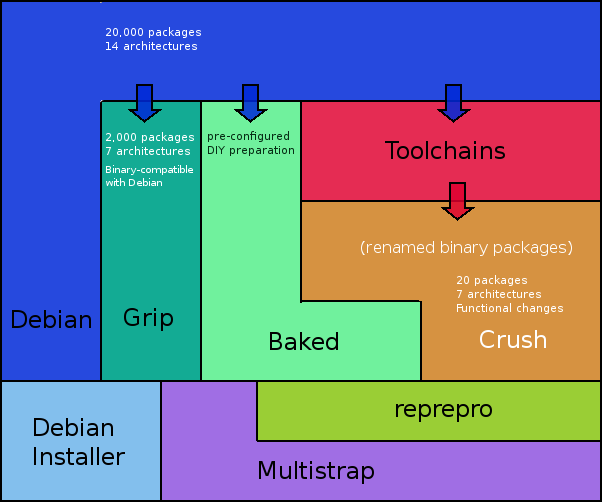
\includegraphics[width=\textwidth]{afbeeldingen/emdebian_soorten}
	\caption{Verschillende soorten van Emdebian en de respectievelijke installatiemogelijkheden}
	\label{fig:emdebian:flavours}
	\legend{(\url{www.emdebian.org}, 2011)}
\end{figure}

Voor de prototype kiosk zullen we gebruik maken van Emdebian Grip, omdat we zo een klein besturingssysteem bekomen maar toch niet te veel flexibiliteit verliezen: als we een pakket nodig hebben dat zich niet in de Emdebian repositories bevindt, kunnen we dat gewoon afhalen van de officiële Debian servers. Dit is vooral interessant omdat we zo applicaties en pakketten kunnen compileren op het toestel zelf, want de Emdebian repositories bevatten niet zoveel development packages. Het alternatief zou bestaan uit het opzettne van een \emph{cross-development environment} op een andere computer, wat vrij veel werk is.
Eenmaal de ontwikkeling van de nodige pakketten voltooid is, kunnen we voor de overige devices gerust gebruik maken van Emdebian Crush of zelfs Baked, aangezien we dan gewoon de pakketten die we reeds op de prototype kiosk gecompileerd hebben moeten installeren.

Zoals figuur \ref{fig:emdebian:flavours} duidelijk maakt kunnen we de verschillende Emdebian basissystemen op verschillende manieren aanmaken. Aangezien we in eerste instantie gebruik zullen maken van Emdebian Grip maar later eventueel wel willen kunnen overschakelen naar Emdebian Crush, zullen we moeten gebruik maken van \code{multistrap} (of zijn voorganger \code{debootstrap}) om het basissysteem samen te stellen. Om multistrap te gebruiken moeten we een configuratiebestand voorzien dat informatie bevat over de pakketten die geïnstalleerd moeten worden. Multistrap zal dit bestand inlezen, alle afhankelijkheden oplossen, en een basissysteem met al deze pakketten genereren.

Maar enkel een basissysteem met de nodige pakketten volstaat niet, we moeten nog verschillende aspecten van het systeem configureren. Daarbij denken we aan netwerkinstellingen, de hostname, welke terminals actief moeten zijn, en welke modules moeten ingeladen worden. Ook kunnen we het resulterende bestandssysteem niet zomaar op een geheugenkaart plaatsen: de partities moeten zodanig aangemaakt zijn dat we vanuit de bootloader exact kunnen verwijzen naar de geheugenadressen van relevante bestanden, \code{uImage} en \code{uInitrd}.

Het is wellicht duidelijk dat dit allemaal geen eenvoudig klusje is. Om zoveel mogelijk te automatiseren en zo menselijke fouten te vermijden, hebben we alle taken beschreven in deze paragraaf gebundeld in \makeurl{https://github.com/MIRAvzw/adastra3-scripts/tree/master/rootfs}{een aantal scripts} die aan de hand van enkele intuïtieve configuratiebestanden het basissysteem volledig autonoom samenstellen.

\subsection{Repository}
\label{kiosk:deployment:besturingssysteem:repository}

Een van de sterktes van Debian is zijn krachtig pakketbeheersysteem. Aangezien we libraries en applicaties gebruiken die zich niet in de standaard Debian repositories bevinden (zoals de kioskapplicatie zelf), moeten we zelf voorzien in een repository met die pakketten in. Hoewel dit niet echt vereist is (zo is het mogelijk om de libraries en applicaties buiten het pakketbeheersysteem om te installeren), heeft dit twee grote voordelen: we kunnen er eenvoudig de software op alle kiosken mee updaten, en het laat toe om het genereren van een volwaardig besturingssysteem volledig te automatiseren met de scripts die we geschreven hebben voor het genereren van het basissysteem.

Vooraleer we een repository kunnen maken, moeten we de code van alle benodigde projecten zodanig verpakken dat de Debian package manager er mee overweg kan. Conversie van een codebase gebeurt met de \code{dpkg-buildpackage} tool, die de code compileert en in een pakketbestand giet aan de hand van een aantal specifieke configuratiebestanden. Zo bevat het \code{control} bestand (zoals er een te zien is in fragment \ref{lst:debian:rules}) essentiële informatie over het pakket: naam, beschrijving, versie, afhankelijkheden, \ldots Een ander belangrijk bestand is het \code{rules} bestand, dat voorschrijft hoe het project geconfigureerd en gecompileerd moet worden. Voor de volledige lijst aan bestanden verwijzen we naar de \makeurl{http://www.debian.org/doc/debian-policy/ch-source.html}{Debian Policy Manual}.

\begin{lstlisting}[float, caption=Debian control packaging bestand., label=lst:debian:rules]
Source: aa3client
Maintainer: Tim Besard <tim.besard@gmail.com>
Homepage: https://sites.google.com/site/miraadastraiii/
Priority: extra
Build-Depends: debhelper (>= 7.0.50~),
               qt4-qmake, libqt4-dev, libbrisa-dev,
               liblog4qt-dev, libsvnqt2-dev, pkg-config
Standards-Version: 3.8.4
Vcs-Git: git://github.com/MIRAvzw/adastra3-client.git
Vcs-Browser: https://github.com/MIRAvzw/adastra3-client

Package: aa3client
Section: lib
Architecture: any
Depends: libqt4-core, libqt4-gui, libqt4-webkit,
         libbrisa, liblog4qt, libsvnqt2,
         ${misc:Depends}, ${shlibs:Depends}
Description: Ad-Astra III client application

Package: aa3client-dbg
Section: libdevel
Architecture: any
Depends: libbrisa (= ${binary:Version}), ${misc:Depends}
Description: Ad-Astra III client application
             (debug symbols)
\end{lstlisting}

Om de gegenereerde pakketten toegankelijk te maken voor het Debian pakketbeheersysteem, moeten we ze onderbrengen in een repository. Dit is eigenlijk niet meer dan een heel exacte bestandshiërarchie, uitgebreid met enkele metabestanden die informatie bevatten over de aanwezige pakketten. Er bestaan verschillende tools om een repository aan te maken, waarbij er enorme verschillen zijn in de mogelijkheden. Omdat onze repository slechts enkele pakketten gaat bevatten, en louter voor intern gebruik dient, kiezen we voor een van de meest eenvoudige tools: \code{apt-ftparchive}. Deze applicatie doet eigenlijk niet veel meer dan het aanmaken van de nodige metabestanden, gebaseerd op een configuratiebestand met alle instellingen erin. Het aanmaken van de exacte bestandshiërarchie met de pakketten op de juiste plaats is de verantwoordelijkheid van de gebruiker, \code{apt-ftparchive} maakt enkel de nodige metabestanden aan. Fragment \ref{lst:debian:repo} illustreert de bestandshiërarchie van een repository met een enkel pakket in.

\begin{lstlisting}[float, caption=Bestandshiërarchie in een Debian repository., label=lst:debian:repo]
debian
|-- dists
|   +-- squeeze
|       |-- Release
|       |-- dev
|       |   |-- binary-armel
|       |   |   |-- Packages
|       |   +-- source
|       |       |-- Packages
|       |       +-- Sources
|       +-- main
|           |-- binary-armel
|           |   |-- Packages
|           +-- source
|               |-- Packages
|               +-- Sources
+-- pool
    |-- dev
    |   |-- aa3client-dbg_0.1-1_armel.deb
    +-- main
        |-- aa3client_0.1-1.dsc
        |-- aa3client_0.1-1.tar.gz
        |-- aa3client_0.1-1_armel.changes
        +-- aa3client_0.1-1_armel.deb
\end{lstlisting}

Tenslotte moeten we de repository nog publiceren, wat kan via een aantal protocollen. We hebben gekozen voor het \ac{ftp}, omdat dergelijke functionaliteit reeds ingebouwd is in het besturingssysteem van de Synology DS207+, de \ac{nas} die we gebruiken als server.

Een repository samenstellen met al zijn pakketten erin is opnieuw een vrij complex en foutgevoelig proces. Daarom hebben we weer zoveel mogelijk proberen te automatiseren met \makeurl{https://github.com/MIRAvzw/adastra3-scripts/tree/master/packages}{een aantal scripts}, die volledig autonoom broncode van projecten kunnen ophalen, er pakketten van maken, ze bundelen in een repository, en finaal die repository deployen op een externe server.

\section{Versioning}
\label{kiosk:deployment:versioning}

Ook voor de kioskapplicatie maken we gebruik van het Git versioning systeem; wat we in sectie \ref{server:deployment:versioning} beschreven hebben is dus hier ook van toepassing.

\section{Compilatie}
\label{kiosk:deployment:compilatie}

Om de software te compileren maken we gebruik van de tools die het Qt framework daartoe biedt. De belangrijkste daarvan is \code{qmake}, een applicatie die het genereren van een \code{Makefile} automatiseert. Dit is vooral interessant omdat, zoals hierboven vermeld, bronbestanden die gebruik maken van Qt-macro's eerst moeten voorverwerkt worden door de \ac{moc} preprocessor. Door gebruik te maken van \code{qmake} moeten we dit niet langer manueel doen: \code{qmake} detecteert welke bestanden eerst moeten verwerkt worden door de preprocessor, en genereert een \code{Makefile} waarbij dit dan ook eerst gebeurt.

Ook hebben we tijdens de ontwikkeling van de applicatie gebruik gemaakt van \makeurl{http://clang.llvm.org/}{Clang}, een moderne compiler voor C en C++. Hoewel deze vrij jonge compiler nog niet op hetzelfde niveau staat als de \ac{gcc}, is het op enkele vlakken veel beter dan \ac{gcc}. Zo is er zeer veel aandacht besteed aan het error reporting subsysteem, waardoor de foutmeldingen die Clang genereert vaak een pak behulpzamer zijn dan wat \ac{gcc} in eenzelfde situatie zou laten weten. Toch worden de uiteindelijke executables gegenereerd met \ac{gcc}, omdat die op vlak van optimalisaties (zowel op vlak van snelheid als grootte) nog steeds de beste keuze is.

Tenslotte is het nog het vermelden waard dat alle libraries die we gebruiken dynamisch gelinkt worden met de finale executable. Dit betekent dat de libraries op het systeem aanwezig moeten zijn, en niet met de applicatie gebundeld worden. Bij de serverapplicatie hebben we dit net anders gedaan, zoals beschreven in sectie \ref{server:deployment:compilatie} hebben we daar alles gebundeld tot een enkel monilitisch geheel. De redenering hierachter is tweeledig. Enerzijds is een kiosk veel statischer: eenmaal we het besturingssysteem samengesteld hebben en er alle nodige applicaties op geïnstalleerd hebben zullen we er lange tijd af blijven. Bij de server is dat anders, niet alleen kunnen en zullen we vaker van hardware veranderen (waarbij vervolgens het besturingssysteem vernieuwd moet worden), ook kunnen we het ons bij een genetwerkte server uit veiligheidsoverwegingen niet veroorloven om jaren aan een stuk dezelfde software te gebruiken. Anderzijds verschillen ook de beschikbare voorzieningen om code in gedeelde bibliotheken af te zonderen: bij C++ code is dit bijvoorbeeld heel eenvoudig dankzij de ingebouwde en sterk geïntegreerde \emph{dynamic linker}. Voor Java applicaties is dit niet het geval: archieven kunnen op arbitraire plaatsen terechtkomen en er zijn geen algemeen aanvaarde mechanismen om die locaties eenduidig te ontdekken en op te vragen bij het opstarten van een applicatie.
